\begin{enumerate}[label=\alph*)]
    \item
        是凸函数, 理由如下:

        $\forall x_1,x_2\in\mathbb{R}$, $\lambda\in[0,1]$, 则
        \begin{align*}
            g(\lambda x_1+(1-\lambda)x_2)
            &=\max_{1\leq i\leq n, i\in\mathbb{Z}}\{f_i(\lambda x_1+(1-\lambda)x_2)\} \\
            &\leq\max_{1\leq i\leq n, i\in\mathbb{Z}}\{\lambda f_i(x_1)+(1-\lambda)f_i(x_2)\} \\
            &\leq\lambda\max_{1\leq i\leq n, i\in\mathbb{Z}}f_i(x_1)+(1-\lambda)\max_{1\leq i\leq n, i\in\mathbb{Z}}f_i(x_2) \\
            &=\lambda g(x_1)+(1-\lambda)g(x_2),
        \end{align*}
        因此$g(x)$是凸函数.

    \item
        不是凸函数, 理由如下:

        \begin{figure}[ht]
            \centering
            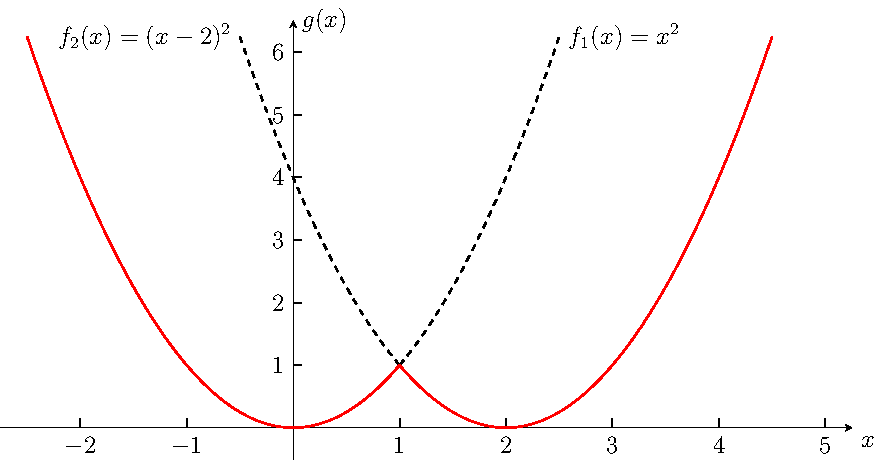
\includegraphics[scale=0.6]{figures/3b.pdf}
            \caption{}
            \label{figure:3b}
        \end{figure}
        如\cref{figure:3b}所示, 取$g(x)=\min\{x^2,(x-2)^2\}$, 即图中红色部分.
        $\forall x_1,x_2\in[0,2]$时,
        \begin{equation*}
            g(\lambda x_1+(1-\lambda)x_2)\geq\lambda g(x_1)+(1-\lambda)g(x_2),\quad \lambda\in[0,1],
        \end{equation*}
        因此$g(x)$不是凸函数.

    \item
        是凸函数, 理由如下:

        $\forall \bm{x}^{(1)},\bm{x}^{(2)}\in\mathbb{S}$, $\mathbb{S}=\left\{[x_1,x_2,\cdots,x_n]^\mathrm{T} \left| ~ x_i>0, \sum_{i=1}^n x_i=1\right.\right\},\lambda\in[0,1]$, 有
        \begin{align*}
            \mathrm{LHS}
            &=g\left(\lambda\bm{x}^{(1)}+(1-\lambda)\bm{x}^{(2)}\right) \\
            &=\sum_{i=1}^n\left(\lambda x_i^{(1)}+(1-\lambda)x_i^{(2)}\right)\log\left(\lambda x_i^{(1)}+(1-\lambda)x_i^{(2)}\right),
        \end{align*}
        \begin{align*}
            \mathrm{RHS}
            &=\lambda g\left(\bm{x}^{(1)}\right)+(1-\lambda)g\left(\bm{x}^{(2)}\right) \\
            &=\lambda\sum_{i=1}^n x_i^{(1)}\log x_i^{(1)}+(1-\lambda)\sum_{i=1}^nx_i^{(2)}\log x_i^{(2)}.
        \end{align*}
        令$h(x)=x\log x$, 易知$h''(x)=\frac{1}{x}>0$, 则$h(x)$为凸函数, 因此有
        \begin{equation*}
            h(\lambda x_1+(1-\lambda)x_2)\leq\lambda h(x_1)+(1-\lambda)h(x_2),
        \end{equation*}
        则
        \begin{align*}
            \mathrm{LHS}
            &\leq\sum_{i=1}^n\lambda x_i^{(1)}\log x_i^{(1)}+(1-\lambda)x_i^{(2)}\log x_i^{(2)} \\
            &=\mathrm{RHS},
        \end{align*}
        因此$g(x)$是凸函数.

    \item
        不是凸函数, 理由如下:

        \begin{figure}[ht]
            \centering
            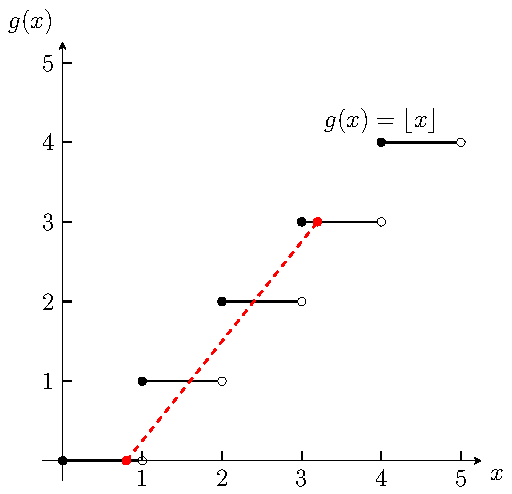
\includegraphics[scale=0.8]{figures/3d.pdf}
            \caption{}
            \label{figure:3d}
        \end{figure}
        如\cref{figure:3d}所示, 取$g(x)$上的点$(0.8, 0)$和$(3.2, 3)$并连成如图中所示的红色虚线段, 可观察到在$[0.8,3.2]$中有存在于线段上方的值, 因此$g(x)$不是凸函数.

    \item
        是凸函数, 理由如下:

        函数$g(x)$可等价地表示为
        \begin{equation*}
            g(x)=\max_{S\subseteq\mathbb{Z}\cap[1,n]\atop |\mathcal{S}|=k}\sum_{x\in\mathcal{S}}x_i.
        \end{equation*}
        又因为$f_1(x)=\max x$与$f_2(x)=x$均为凸函数, 则$g(x)$也为凸函数.

    \item
        是凸函数, 理由如下:

        $\forall x_1,x_2\in\mathbb{R},\lambda\in[0,1]$, 有
        \begin{align*}
            \mathrm{LHS}
            &=g(\lambda x_1+(1-\lambda)x_2) \\
            &=(\lambda x_1+(1-\lambda)x_2)^2 \\
            &=\lambda^2 x_1^2+(1-\lambda)^2x_2^2+2\lambda(1-\lambda)x_1x_2,
        \end{align*}
        \begin{align*}
            \mathrm{RHS}
            &=\lambda g(x_1)+(1-\lambda)g(x_2) \\
            &=\lambda x_1^2+(1-\lambda)x_2^2,
        \end{align*}
        \begin{align*}
            \mathrm{LHS}-\mathrm{RHS}
            &=\left[\lambda^2 x_1^2+(1-\lambda)^2x_2^2+2\lambda(1-\lambda)x_1x_2\right]-\left[\lambda x_1^2+(1-\lambda)x_2^2\right] \\
            &=-\lambda(1-\lambda)(x_1+x_2)^2 \\
            &\leq 0,
        \end{align*}
        因此$g(x)$是凸函数.
\end{enumerate}
